\section{Errors in relational data}
% How are errors typically classified, identified etc..
% What are common type of approaches to find errors automatically
The perspective in this research is about comparing two versions of the data. One "dirty" dataset and one "clean" dataset. Values from the "dirty" version that are not equal to their "clean" counterparts, are counted as errors. These errors come in all different types, in terms of content or methods of detection. Also, different metrics or scores can be used to evaluate the found errors or to analyze a "dirty" dataset compared to the "clean" version.
 
In the following subsections, different error types and metrics to evaluate error detection methods will be discussed. Also test datasets and synthetic error generation are discussed to sketch a more complete view of the current error detection environment in research.

\subsection{Error types}
\label{subsec:errortypes}
In research, errors have been described with error types. A compilation of these types can be find in the survey by \cite{Abedjan2016-jc}. It gives the following types as broad categories for errors:
\begin{itemize}
    \item Outliers
    \item Duplicates
    \item Rule violations
    \item Pattern violations
\end{itemize}

These categories are overlapping and non-exhaustive. The types above mainly describe how the errors can be found, not necessarily how they are introduced. 

% Quantitative
% Outliers
% 1. Outliers include data values that deviate from the
% distribution of values in a column of a table.
\paragraph{Outliers} include data values that deviate from the distribution of values in a column of a table.
\blockquote{Characterizing,
locating, and in some cases eliminating these outliers offers
interesting insight about the data under scrutiny and reinforces
the confidence that one may have in conclusions drawn from
otherwise noisy datasets. \cite{Pit--Claudel2016-dj}}. 

% Qualitative
% Duplicates
% 2. Duplicates are distinct records that refer to the same
% real-world entity. If attribute values do not match, this
% could signify an error
\paragraph{Duplicates} are different tuples, referring to the same real-world entity. If attribute values do not match, this could signify an error in the data, but could also be the result of bad schema design, where redundancy of information is present.

% Rule violations
% 3. Rule violations refer to values that violate any kind
% of integrity constraints, such as Not Null constraints
% and Uniqueness constraints
\paragraph{Rule violations} refer to values that violate any kind of integrity constraints, such as Not Null constraints and Uniqueness constraints.

% Pattern violations
% 4. Pattern violations refer to values that violate syntactic and semantic constraints, such as alignment, formatting, misspelling, and semantic data types.
\paragraph{Pattern violations} refer to values that violate syntactic and semantic constraints, such as alignment, formatting, misspelling, and semantic data types.

% Other
\paragraph{Other errors} include wrong references (\cite{Rahm2000-fz}), wrong content or other types of errors do not fall into the other categories, but are different to the ground truth.

It is also important noting that this research will focus on single-source data error problems (\cite{Rahm2000-fz}). In real world environments, the problems and challenge that arise out of data errors will become more and more complex with a growing number of sources. Fixing errors with a single source as scope is less complex. Also, most error detection methods only support using a single dataset. However, when a single source is cleaned, the detected errors and repair value pairs can be iterated through other sources.

\subsection{Metrics \& Data quality}
\paragraph{Data quality}. A term often used in data cleaning is "data quality". Data quality describes a dataset in a number of dimensions. Depending on the task at hand, these dimensions might differ. The basic set of dimensions is accuracy, completeness, consistency, and timeliness (\cite{Batini2009-aa}). One can refer to either the data values or the schema with regards to the quality. Data quality also gives information about the usability of the data in analysis. If the quality is high, the results of visualizations, aggregate values or other grouped actions are close to the expected results. So higher data quality gives more confidence in using a dataset.

\paragraph{Accuracy}
is the metric consisting of the sum of all true positives and true negatives, divided by the total number of instances. Whenever working with imbalanced datasets, this number could give a misleading confidence in the score, whereas the larger type (positives or negatives) dominates the score.

\paragraph{Precision}
is the metric consisting of the count of all true positives, divided by all the true positives and false positives. This metric is the fraction of relevant instances among all the "detected" positives. High precision means that the quality of errors detected is good, without having a large fraction of false positives. This metric could be helpful for completely automated processes. If precision is 1, no mistakes were made in the detected errors and no human interaction is needed. This metric however does not tell anything about the portion of total errors retrieved and errors still left in the dataset, only about the quality of the instances predicted to be errors.

\paragraph{Recall} 
is the metric consisting of the count of all true positives, divided by the count of all true positives and false negatives. Whereas precision measures the quality of positively labeled instances, recall is the fraction of correctly detected errors divided by the total number of true errors in the dataset. This metric focuses on retrieving all errors from the dataset, without any regard for the quality of the predictions.

\paragraph{F1-score}
is the metric that is the harmonic mean of precision and recall. So it is a combination of both recall and precision, measuring each score with equal importance. Due to this mix of importance, it is usable as a single metric, while having a larger scope of measurement.
% ~\\The F1-score (also F-measure), will be the main goal to estimate in later sections.

% What are important things in the automated error detection field
\subsubsection{Automation}
Depending on the error detection task at hand, a metric from the list above could be selected to rate the error detection method. For automating the error detection task, high precision could be emphasized. 
Like discussed by \cite{Huang2018-er}, for automatically detecting errors, the aim should be to set a very high bar in terms of
precision, as users would quickly lose confidence if the system keeps
generating spurious alerts. Methods that achieve higher recall could be useful in scenarios where manual checking after detection is done, to ensure higher coverage, but at a higher human cost.

\subsubsection{Benchmarks \& Evaluation}
Public benchmark methods for error detection and data cleaning in relational data sources have been scarce. 
\paragraph{CleanML (\cite{Li2019-ve})} investigates the impact of data cleaning on downstream machine learning models. Besides providing numerous datasets for testing, it focuses on the impact of cleaning separate error types on the end machine learning task. It tackles the following error types:
\begin{enumerate}
    \item Inconsistencies
    \item Duplicates
    \item Mislabels
    \item Outliers
    \item Missing Values
\end{enumerate}
Types 2, 3 and 5 are known from other research, whereas inconsistencies and mislabels are more niche category descriptions. Inconsistencies can be covered as rule violations and mislabels would fall under the "Other errors" from section \ref{subsec:errortypes}. Unfortunately, this method does not cover holistic data cleaning. Due to the high overlap in both the descriptions of error types, in combination with treating single error types separately, it cannot properly tackle the task at hand in this thesis.

\paragraph{Data quality estimation} is a way of evaluating the results of a cleaning method, without knowing the ground truth. The research by \cite{Chung2017-cl} shows a method to estimate data quality, by letting a human iteratively judge parts of the data, to get a good estimate of the accuracy and quality, without having access to the ground truth beforehand. Its main point of view is estimating the number of errors based on the initial "dirty" dataset. This aligns with the goals of this thesis. However, because the ground truth is known for all the used datasets and due to the stochastic nature of this method, it is not suited for the empirical study in the upcoming sections. This concept might be used as an extension to this work, when adding larger datasets where the ground truth is not known beforehand.

% Mogelijk nog de automatische data quality verwerken \cite{Schelter2018-au}

\subsection{Datasets \& Error generation}
In contrary to the limited number of benchmark methods in data cleaning, there have been many efforts to publish clean and dirty dataset pairs, to be used for evaluating error detection and repairing methods. Also, it has been used in research to synthetically introduce errors in datasets that were clean beforehand.

\subsubsection{Datasets}
A list of datasets extracted from different papers and researches will be used in this thesis. There are multiple ways of communicating a dirty version of a dataset and its ground truth counterpart. The most useful way for this research of denoting a dataset and its ground truth is explained by \cite{Mahdavi2019-zf}. A clean and dirty version are handled as deterministic and known values. The datasets will be provided by 2 different files (or in-memory tables), like depicted in figures \ref{fig:dirtydataset} and \ref{fig:cleandataset}. Whenever such a dirty-clean dataset pair is used, it is assumed to be correct. The difficulty of data cleaning lies in the ambiguity of what the ground truth might be. 

\begin{figure}[h]
\centering
\begin{subfigure}[b]{0.75\textwidth}
   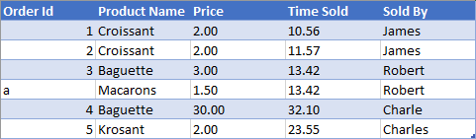
\includegraphics[width=\linewidth]{thesis/Figures/DirtyDataset.png}
   \caption{A dirty dataset d}
   \label{fig:dirtydataset} 
\end{subfigure}

\begin{subfigure}[b]{0.75\textwidth}
   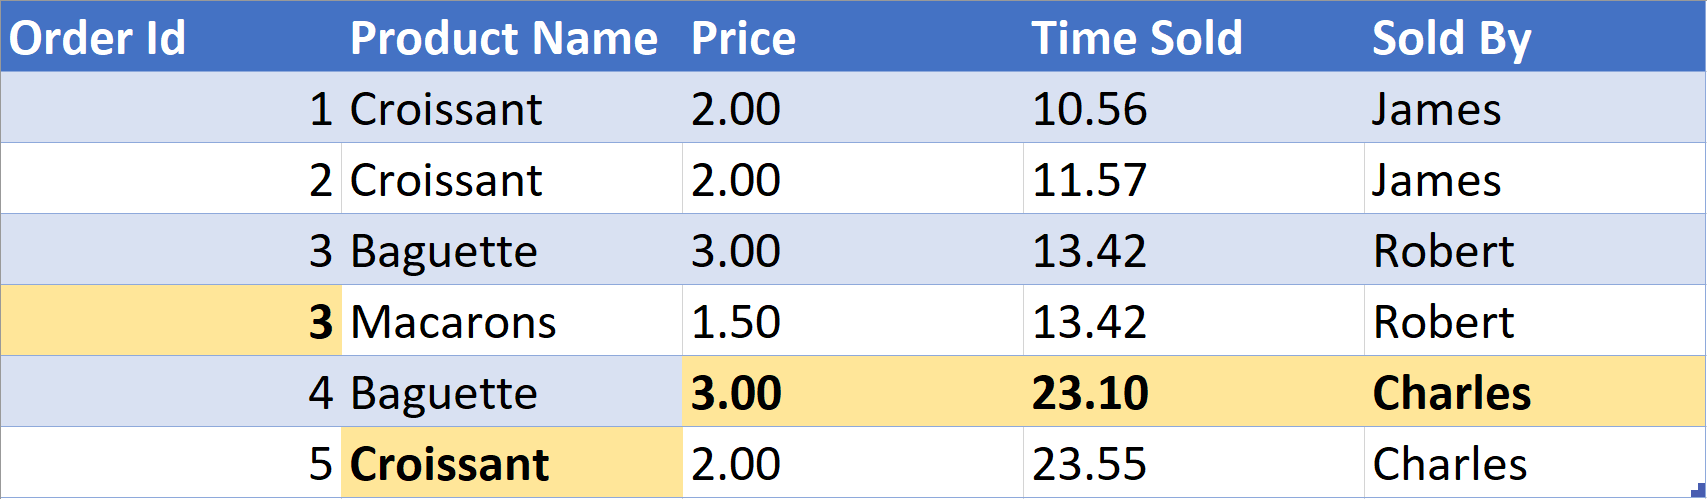
\includegraphics[width=\linewidth]{thesis/Figures/CleanDataset.png}
   \caption{Its ground truth d*}
   \label{fig:cleandataset}
\end{subfigure}
\caption{A dirty-clean dataset pair}
\end{figure}

Other research provides errors in other structures. For example, with MDedup (\cite{Koumarelas2020-oz}), dirty datasets are provided. Separately, files with duplicate rows are provided, stating each source row id and duplicate row id. 

CleanML (\cite{Li2019-ve}) provides separate clean and dirty datasets for each different error type. For this thesis, error detection tools will be evaluated holistically, meaning that the dirty and clean dataset should include all different error types in one version. To merge the split versions, the dirty datasets are merged together, as the ground truth stays the same for all versions. This will leave 2 datasets, one dirty and one clean.

% Hier over wat voor dirty vs clean er worden gegeven in de research
% BigDaMa groep
% CleanML combining errors

\subsubsection{Error generation}
To evaluate all error detection tools, a ground truth needs to be known and errors need to exist in the dirty dataset. 

\paragraph{Crowd sourcing \& Expert labeling}
To generate dirty-clean dataset pairs, real life dirty datasets can be used and corrected by experts. This is a timely and costly process, with increasingly higher complexity with growing datasets. The cost of labeling causes a limited number of train and test datasets for this research field.
The work presented by \cite{Sheng2008-gk} shows that repeated labeling can improve the data quality for supervised learning. Even when the individual accuracy of labeling from crowdsource labelers is not 100\%, it is possible to generally retrieve higher quality labels than a single labeler would generate. Repeated labeling could be a way of creating the ground truth from a real world dataset, by letting users correct cells in a given dataset.

\paragraph{Synthetic errors} To circumvent the high costs of labeling, BART (\cite{Arocena2015-om}) was proposed to synthetically introduce detectable errors into clean datasets. The error-generation problem was shown to be NP-complete. The authors made a distinction between detectability and repairability. When introducing errors into a dataset, it is important that generated new values can actually be considered errors. Therefore, a user of BART must provide certain constraints on the data to specify when and if a value is a violation. Also, the user can then provide the portion of the dataset that should be turned into errors. 
Besides the evaluation of error detection tools, BART can also be used to measure error correction (repair) tools. Whenever an error is introduced, it is known whether or not this value lies in the specified domain of values and if the ground truth value can be found in other parts of the data. If this is not the case, the repairability decreases, as it is a hard process to find the ground truth. However, repairing is outside the scope of this thesis and the main focus will lie on the error generation with detection as the priority task. 